\section{Patientforløb med hypertension}
Med udgangspunkt i Leavitts modificerede organisationsmodel, ses hvilke påvirkninger der forkommer i modellens fem områder ved implementering af Fitbit Flex. Dertil ses hvilken virkning teknologien har på behandlingsforløbet.

\subsection{Diagnose og udredning af hypertension} \label{sec:dia_hypertension}
Som beskrevet i \autoref{sec:hypertension} ses der sjældent symptomer ved hypertension og opdages derfor ofte ved en tilfældighed ved eksempelvis sundhedstjek hos patientens alment praktiserende læge. 
Diagnosen hypertension kan ikke stilles på baggrund af én blodtryksmåling foretaget hos lægen, da patienten kan være nervøs og derved have et højere blodtryk og påvirke resultatet. Patienten bør få foretaget enten døgnblodtryksmåling eller hjemmeblodtryksmåling, hvis målinger i klinikken viser forhøjet blodtryk. Patienten kan desuden sidde i et rum uden tilstedeværelse af sundhedspersonale og få foretaget blodtryksmålinger med en automatisk blodtryksmåler \citep{lodberg2016, bech2015}.

En hypertensionskontrol består af forskellige  undersøgelser. I rapporten \citetalias{munck2007} blev personalet spurgt om hvilke områder hypertensionskontrollen bestod af. I over 50 \% af de deltagende praksis omhandlede kontrollen, en blodtrykskontrol, en vægtkontrol, information omkring rygeafvænning, kostvejledning og vejleding omkring motion og fysisk aktivitet. Data fra studiet oplyste yderligere at 79,9 \% af personalet inkluderede instruktion i hjemmeblodtryksmåling ved hypertensionskontrollerne. Dette omhandlede blandt andet instruktion i udfyldelse af et registreringsskema for blodtryksmålingerne \citep{munck2007}. 

Såfremt flere blodtryksmålinger viser et forhøjet blodtryk skal patienten igennem en videre udredning. Patientens tidligere sygehistorie vil tages i betragtning, herunder blandt andet forskellige risikofaktorer for hypertension såsom lavt aktivitetsniveau, diabetes og familiær disposition til blandt andet hypertension, diabetes og nyresygdomme. Foruden dette foretages en objektiv undersøgelse af patienten, hvor blandt andet højde, vægt og abdominalomfang måles. Der tages desuden EKG-målinger, blodprøver og urinprøver, og ved kliniske tegn på hjertesvigt, henvises patienten til sekundærsektor for at få foretaget røntgen af thorax og ekkokardiografi \citep{lodberg2016, bech2015}.

Er den hypertensive patient under $40$ år, har et meget højt blodtryk eller har behandlingsresistent hypertension, bør patienten undersøges for sekundær hypertension for at sikre, at det ikke er en eller flere bagvedliggende sygdomme, der har hypertension som en følge \citep{lodberg2016}. Sekundær hypertension forekommer hos mindre end $5~\%$ af tilfældene, og den hyppigste årsag er nyresygdomme \citep{lodberg2008}. Patienten kan eksempelvis henvises til nefrologisk afdeling for yderligere undersøgelser, hvis der findes eller er mistanke om en bagvedliggende nyresygdom \citep{lodberg2016, sundhedsstyrelsen2010}. 

\subsubsection{Samspil mellem primær og sekundær sektor}
Under udredning og behandling kan hypertensive patienter, hvis nødvendigt, blive henvist til forskellige afdelinger af den alment praktiserende læge. Regionen, hvori patienten er bosat, har betydning for, hvor patienten henvises til. Henvisning kan eksempelvis være til Blodtrykscenteret i Region Midtjylland, hvor Nyremedicinsk, Hjertemedicinsk og Endokronologisk Afdeling i samarbejde behandler hypertension og eventuelle følgesygdomme, samt patienter med sekundære hypertension. Patienter kan henvises til Blodtrykscenteret ved behandlingsresistent hypertension, hypertension i forbindelse med nogle former for hjertekarsygdomme, mistanke om sekundær hypertension eller hvis nyopdaget hypertension skal verificeres ved hjælp af døgnblodtryksmåling. Ved en henvisning til Blodtrykscenteret vil patienten forinden være forsøgt udredt af egen læge, hvor informationer om udredningen vedlægges henvisningen \citep{aarhusuniversitetshospital}. 

I regioner uden et center såsom Blodtrykscenteret vil hypertensive patienter typisk blive henvist til nefrologisk, kardiologisk eller endokronologisk afdeling \citep{buur2011}. Når det vurderes af lægerne på den pågældende afdeling, at patienten har fået den tilstrækkelige behandling og/eller udredning på afdelingen, afsluttes behandlingen, og patienten kan efterfølgende gå til kontrol ved alment praktiserende læge \citep{sundhedsstyrelsen2010, lodberg2016}.

Hvis Fitbit Flex bliver implementeret som en del af behandlingen af hypertension kan dette påvirke strukturen i organisationen ved at ændre antallet af patienter, der bliver henvist til forskellige afdelinger i den sekundære sektor. Hvis aktivitetsarmbåndet har en positiv effekt, og flere patienter opnår reduktion i blodtryk som følge af højere aktivitetsniveau, kan der være færre følgevirkninger såsom nyresygdomme og hjerteproblemer. Hvis ikke dette var tilfældet kunne man i stedet opnå en udskydelse af diverse følgesygdomme. Dette kan resulterer i at færre patienter henvises til den sekundære sundhedssektor. 

\subsection{Behandling af hypertension}

Når den alment praktiserende læge har diagnosticeret og vurderet patienten, kan behandlingen påbegyndes. Behandling af hypertension afhænger af, hvilken grad af hypertension patienten har, samt hvorvidt det er sekundær hypertension. Det er herved forskelligt, hvor og hvem der varetager behandlingen. Opstår følgevirkninger, der kræver yderligere behandling, henvises patienten til en specialiseret afdeling, hvor behandlingen varetages, indtil patienten er stabil og kan fortsætte hypertensionskontrol hos egen læge \citep{sundhedsstyrelsen2010}.

Som skrevet i \autoref{sec:hypertension} har lægen i den almene klinik mulighed for at behandle hypertensive patienter farmakologisk og non-farmakologisk. Behandlingen vurderes ud fra, om patienten har risiko for kardiovaskulær sygdom, hvor lægen blandt andet undersøger om patienten har risikofaktorer såsom hypertensive organskader, diabetes og nyresygdomme \citep{promedicin2016}.

Farmakologisk antihypertensiva-behandling startes, hvis patienten har et blodtryk på over $180$/$110$ mmHg, da det på dette tidspunkt ikke er tilstrækkeligt med omlægning af livsstil, herunder rygestop, motion, kostændringer og saltindtag \citep{pedersen2016, bech2015}. 

\begin{figure}[H]
\centering
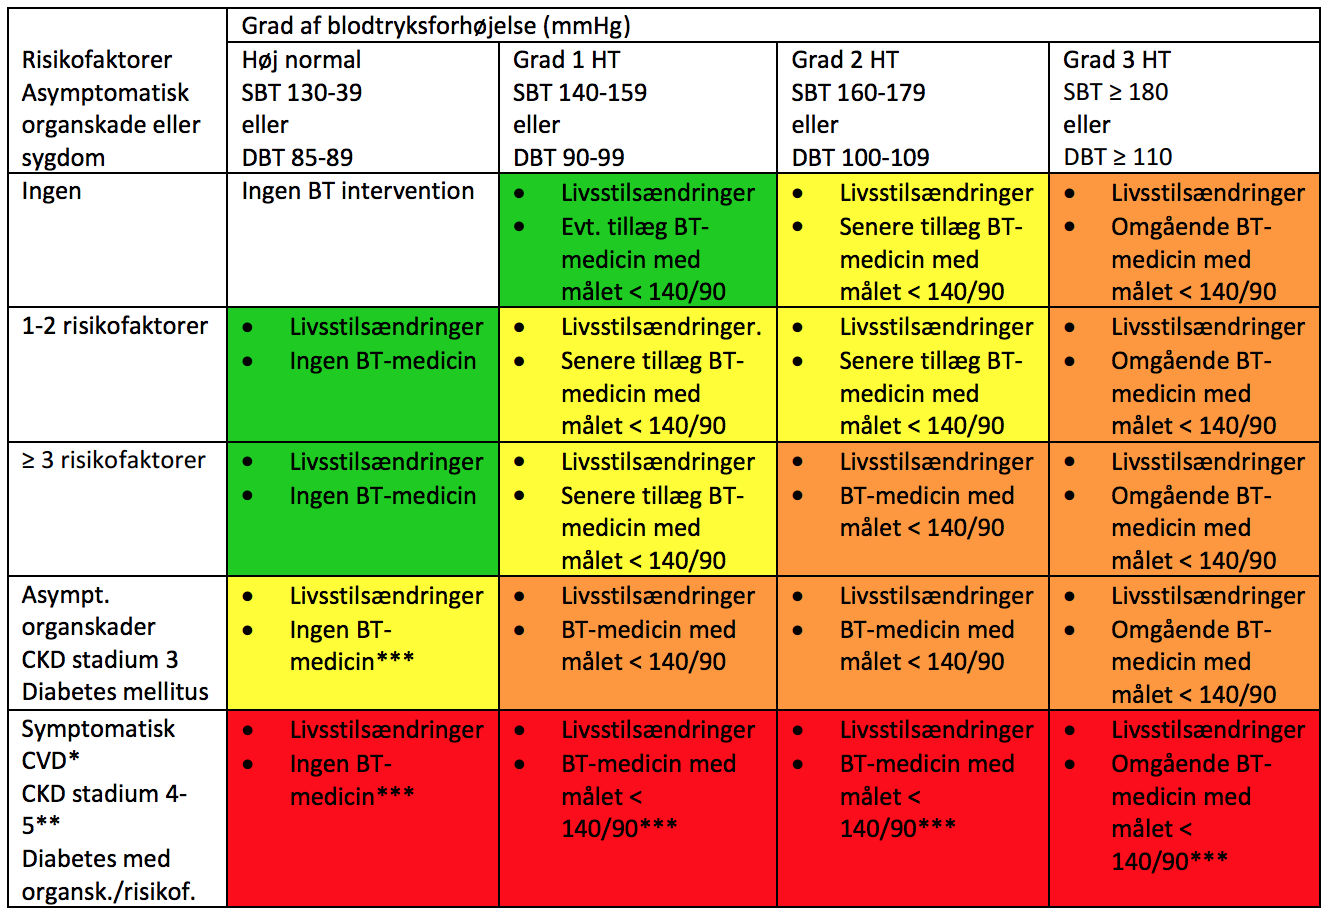
\includegraphics[width=0.9\textwidth]{figures/behandlingsvejl}
\caption{Behandlingstilgang i relation til risikofaktorer og målt blodtryk. $10$ års risiko for apopleksi eller myokardieinfarkt - Rød: meget høj risiko ($>30~\%$), orange: høj risiko ($20-30~\%$), gul: middel risiko ($15-20~\%$) og grøn: lav risiko ($<15~\%$) samt hvilken konsekvens, som bør drages af inddelingen. (HT: hypertension; SBT: systolisk blodtryk; DBT: diastolisk blodtryk). *: CVD (kardiovaskulær sygdom), **: CKD (kronisk nyresygdom), ***: Evt. strammere blodtryksmål hos visse patienter med diabetes og patienter med proteinuri \citep{bech2015}.}
\label{fig:behandlingsvejl}
\end{figure}

\noindent
I \autoref{fig:behandlingsvejl} ses hvilke tiltag der er nødvendige i relation til patientens blodtryk, samt hvilke risikofaktorer patienten er vurderet til at have. Har patienten en mild grad af hypertension, hvilket illustreres med grøn på \autoref{fig:behandlingsvejl}, kan patienten muligvis nøjes med livsstilsændringer, hvis der er få risikofaktorer. Fra middel til meget høj risiko for følgesygdomme af hypertension, illustreret med gul, orange og rød på \autoref{fig:behandlingsvejl}, bør der tillægges blodtryksmedicin \citep{bech2015}.
\citetalias{munck2007} er et projekt ved Forskningsenheden for Almen Praksis i Odense, hvor en rapport er udgivet omhandlende registreringer af hypertension i 184 almene praksisser. Ifølge denne rapport var $35,3~\%$ af de hypertensive patienter for lidt fysisk aktive, og dermed var lavt aktivitetsniveau den tredje hyppigste risikofaktor \citep{munck2007}.

Yderligere var $11~\%$ af de registrerede hypertensive patienter i non-farmakologisk behandling, samtidig var det kun $1,7~\%$ af de registrerede patienter, der ikke fik nogle former for farmakologisk behandling \citep{munck2007}.
 %(Jeg ved ikke hvor jeg er på vej hen… Hjælp. Er alt det her overhovedet relevant at have med? DET ER COOLT MED TAL, HVOR MANGE DER EGENTLIG BLIVER BEHANDLER ALTSÅ HVOR MANGE DER ER REGISTRERET. JA JEG SYNTES OGSÅ AT DET VIRKER MEGET FORNUFTIGT)
Anvendelse af aktivitetsarmbånd til behandling af hypertension vil høre under kategorien non-farmakologisk behandling i form af livsstilsændringer. Hertil vil lægen eller sygeplejersken få til opgave at oplære patienten i brug af armbåndet og siden følge op på aktivitetsniveauet. Lægen kan ud fra data om aktivitetsniveauet vejlede patienten om motion. 
Skulle en stigning af blodtrykket forekomme under behandlingen, kan lægen vurdere, om det kan skyldes et fald i aktivitetsniveau. Ligeledes ville et lavere blodtryk kunne skyldes, at aktivitetsniveauet er steget. Det vil på denne måde være muligt at sammenligne objektive målinger af aktivitetsniveauet med patientens prognose. 

\subsection{Aktivitetsarmbånd i den nuværende organisation}
I relation til Leavitts modificerede organisationsmodel er mulige interessenter for anvendelse af aktivitetsarmbånd, som en del af behandling mod hypertension, de praktisserende læger.

I \citetalias{munck2007} blev personale i almene praksisser adspurgt hvorvidt det ønskes, at personalet involveres mere i patientbehandlingen af hypertension, hvortil $67,3~\%$ svarede ja. Ud af disse svarede omkring $49~\%$, at de ønsker øget involvering indenfor vejledning om motion og fysisk aktivitet \citep{munck2007}. Disse tal kan tyde på, at en stor andel af de almene praksisser kan være åbne for nye muligheder eller forbedringer inden for vejledning om fysisk aktivitet i forbindelse med hypertension. Ved indførelse af Fitbit Flex som en del af behandlingen af hypertension har personalet i den almene praksis mulighed for at monitorere patientens fysiske aktivtetsmønster og kan dermed få bedre mulighed for at tilpasse vejledningen til patienten. 

Andre mulige interessenter kan også være læger og andet personale i den sekundære sektor. Blodtrykscenteret i Region Midtjylland reklamerer blandt andet med, at forskning og implementering af nye behandlingsmetoder foregår med udgangspunkt i Blodtrykscenteret \citep{aarhusuniversitetshospital}. Foruden dette kan afdelinger på sygehuse, der behandler mange hypertensive patienter, have interesse i at få implementeret behandlingen i de almene klinikker. Hvis antallet af svære tilfælde af hypertension reduceres, kan det dermed påvirke samspillet mellem primær og sekundær sektor. 

Yderligere fungerer læger og sygeplejersker i almen praksis også som aktører, da de vil få til opgave at lære at anvende aktivitetsarmbånd som en del af et behandlings- og monitoreringsforløb for hypertensive patienter. 
Indførelse af aktivitetsarmbånd kræver derfor, at de alment praktiserende læger ønsker at innovere behandlingen og anvende den alternative behandlingsmetode i klinikkerne. Nogle vil muligvis være skeptiske over for indførelse af en ny teknologi, såsom Fitbit Flex. De læger, der har interesse i at benytte aktivitetsamrbånd i form af Fitbit Flex, kan indføre det i praksis. Har indførelsen en positiv effekt, kan teknologien udvides til flere alment praktiserende klinikker, hvis disse ændrer mening.

For at gøre det mere attraktivt for de praktiserende læger at anvende en ny teknologi, der kræver omstilling i forhold til den almindelige arbejdsgang, kan der indføres et honorar for anvendelse af aktivitetsarmbånd som en del af behandlingen for hypertension. Ved at honorere anvendelse af nye teknologier i almen praksis, kan anvendelsen af udstyret øges, hvilket eksempelvis har gjort sig gældende ved hjemmeblodtryksmåling \citep{bang2006}.